\label{app:ferr_Prop}

For any cavity which possesses resonant modes, it is possible to describe it's impedance by using a set of physical parameters. Each mode may be characterised by its resonant frequency $f_{res}$, its quality factor $Q$, its shunt impedance $R_{s}$ and the parameter $R_{s}/Q$. These parameters are dependent on the geometry of the structure, and the materials that make up the surfaces and volume spaces within it. It is generally possble to consider these parameters by either evaulating the fields within the structure, or by comparison to equivalent circuit model of the cavity (a simple example of which is shown in Fig.~\ref{fig:cavCircuitModel}. More complex circuit models exist for calculating coupled cavities \cite{Knapp:CoupledResModel} defined by a resistance $R_{s}$, a capacitance $C$ and an inductance $L$.

\begin{figure}
\begin{center}
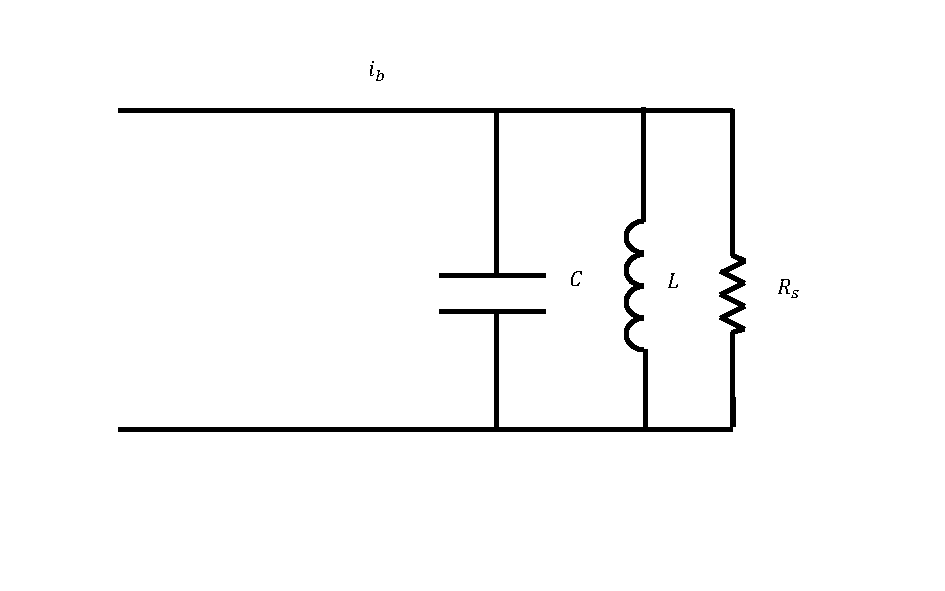
\includegraphics[width=0.6\textwidth]{appendices/figures/equiv-circuit.pdf}
\end{center}
\caption{The equivalent circuit model for a cavity mode with no coupling to neighbouring cavities.}
\label{fig:cavCircuitModel}
\end{figure}

The capacitance and inductance of the circuit representation are related to the resonant frequency by

\begin{equation}
2\pi f_{res} = \omega_{res} = \frac{1}{\sqrt{LC}}.
\end{equation}

The quality factor $Q$ is defined as

\begin{equation}
Q = \frac{\omega_{res}W}{P_{surf}} = R_{s}\sqrt{\frac{C}{L}}
\end{equation}

considering the cavity parameters and circuit representation respectively. The shunt impedance $R_{s}$ is defined as

\begin{equation}
R_{s} = \frac{V_{acc}^{2}}{P_{surf}}
\end{equation}

where $V_{acc}$ is the potential that a traversing particle experiences, given by

\begin{equation}
V_{acc} = \int^{L}_{0} E_{z} e^{j\omega z/c} dz.
\end{equation}

A useful relationship to know regarding the quality factor is that due to the losses in the cavity being dependent on the conductivity of the wall material, for any given cavity the quality factor of a cavity made of material $c$, $Q_{c}$ with a conductivity $\sigma_{c}$ compared to the same cavity made from material $d$, with conductivity $\sigma_{d}$ giving a quality factor $Q_{d}$, is given by

\begin{equation}
Q_{c} = \sqrt{\frac{\sigma_{c}}{\sigma_{d}}}Q_{d}
\end{equation}

for the case where there is no significant quantity of lossy material in the structure. For cases of strong damping by the inclusion of lossy material this no longer holds true.

For any given eigenmode solution in an eigenmode solver in a computational electromagnetic solver (for instance Ansoft HFSS) the default results produced are the eigenfrequency $f_{res}$ and the electromagnetic field pattern of the mode. $Q$ is also given if a lossy material (either a finite conductvity or a material with dielectric or magnetic losses)  is defined within the simulation volume. It is possible to calculate the $R_{s}/Q$ of the resonance by evaluating the fields of the resonance, either using the internal calculator of the programme or by exporting the fields necessary and using an external script/code.

\section{Longitudinal $R_{s}/Q$}

For a structure, the longitudinal $R_{s}/Q$ of the mode is defined by

\begin{equation}
\frac{R_{s}}{Q}_{\parallel} = \frac{V_{acc}^{2}}{\omega_{res} W} = \frac{\left| \int^{\infty}_{\infty} E_{z} \left( x,y,z \right) e^{j \omega_{res}z/\left( \beta c \right)} dz \right|^{2}}{\omega_{res} W}. 
\end{equation}

From HFSS we acquire a discrete field pattern due to the finite mesh, thus it is necessary to use a discrete integration method to calculate this from simulation results. The choice of algorithm for this is largely left to the user to decide.

It should be noted that the longitudinal $R_{s}/Q$ is dependent on the beam displacement and path through the locale of the eigenmode, thus the beam path should be considered during the analysis, especially for devices where multiple possible beam paths exist.

\section{Transverse $R_{s}/Q$}

The transverse $R_{s}/Q$ of an eigenmode can be calculated in two seperate ways. Using the similar definition of the longitudinal $R_{s}/Q$ but for the transverse fields, the transverse $R_{s}/Q$ for a particle displaced in the x direction (for the y-plane the field components are swapped $x \rightarrow y$, $y \rightarrow x$) is given by \cite{Grudiev:LongTransSecCol}

\begin{equation}
\frac{R_{s}}{Q}_{\perp} = \frac{c \left( \int^{\infty}_{\infty} \frac{\partial E_{z} \left( x,y,z \right)}{\partial z} e^{j \omega_{res}z/\left( \beta c \right)} dz\right)^{2}}{\omega_{res}^{2}W} = \frac{ \left( \int^{\infty}_{\infty}  \left( E_{x} \left( x,y,z \right) + c B_{y} \left( x,y,z \right) \right) e^{j \omega_{res}z/\left( \beta c \right)} dz\right)^{2}}{cW}.
\end{equation}

It can be seen that $(R_{s}/Q)_{\perp}$ is dependent on the transverse displacement of the beam as with $(R_{s}/Q)_{\parallel}$. For small displacements this dependence on the transverse position can be considered to be linear in non-extreme cases (i.e. far from any material boundaries/non-linear materials) and thus a transverse $R/Q$ normalised to displacement used.
